by Pavlo Kravets


Different segments of the market require different strategies to capture value effectively. Our possible B2B customers would have different motivations, requirements and resourses than our B2C customers. As such, we need to rely on different business models.

\section{B2C}

For the B2C market we are employing a Freemium business model. We are separating our B2C customers into 2 groups: the subscribers and the free users.

Free users will be periodically shown interstitial ads, while the subscribers will have ad-free experience. Interstitial ads vary in price quite a lot: the price depends on customers location, platform, current market demand, etc. According to the report provided by Marc Llobet Rodriguez\cite{ECPM}, in Q3 of the 2023 the CPM (cost per mille) for interstitial ads in developed countries was between 10 and 16 euros. In our calculations we assume this holds true in the future and use a CPM of 13€.

Subscribers, on the other hand, will not be shown any ads. They will be paying a yearly subscription price instead. The price may be adjusted with various promotions, but we assume that the average yearly subscription price will be 15€. Besides the ads removal, users maz be enticed to subscribe by offering various add-ons and premium features.

One of the key problems in B2C market is customer churn. The 30-day retention rate for healthcare apps was 3.7\% according to research\cite{churn}. As such, yearly subscription has several advantages over the monthly one:
\begin{itemize}
    \item It helps to capture more value from the impulsive purchasers. A healthcare app spending may be driven by an acute problem - for example, a period of intense neck pain. Such customers may cancel monthly subscription after the end of the acute episode
    \item It may lead to a stronger habit. The user may utilize the app more if they have already invested into yearly subscription - which, in turn, makes them more used to the app
    \item Some customers may find a single yearly payment less worrying than a monthly expense. They will have a constant reminder of a positive sides of the app, not of the price they pay for it
\end{itemize}

High rates of customer churn and relatively unknown market leads us to believe that we will see exponential growth in active users during the initial period, which turns to linear as time progresses.

\section{B2B}
For the B2B market, we will be mostly employing subscription and one-time payment models, depending if the business customer would prefer to have support or not.

Other possible revenue stream is selling add-ons and customization packages. A lot of businesses may have unique or semi-unique technical requirements. Those requirements can be priced on case-by-case basis, developed and delivered to the customer.

Most businesses prefer to work with well-established countragents. This, as well as possible huge swings in the earnings depending on customer's size and requirements make estimations extremely imprecise. As such, B2B segment is not taken into concideration for calculating the business plan.

\section{Legal structure}

The legal structure chosen for the company is GmbH. It provides limited liability.

As discussed in chapter \ref{chp:team_structure}, there are 5 founders in the company. It makes no financial sense for those founders to pay themselves salaries out of their own pocket, so they will forego salaries. This makes the expenses much lower, but means that the alternative should be calculated: how much would those people earn working as an employee in another company?

\begin{figure}[H]
    \centering
    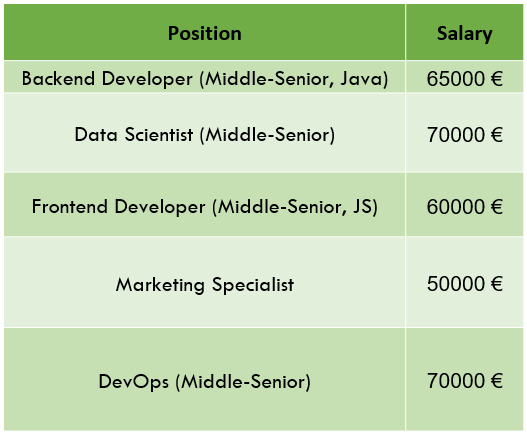
\includegraphics[width=0.5\textwidth]{figures/founder_salaries.png}
    \caption{Founders' foregone salaries}
    \label{fig:founder_salaries}
\end{figure}

In figure \ref{fig:founder_salaries} we can see salaries (brutto) for the position and experience level needed, according to Glassdoor.

\section{Cost structure}

The costs for this project can be classified into two camps: one-time payments and ongoing costs.

There are following one-time payments:

\begin{itemize}
    \item Initial capital for GmbH - 25000€
    \item Initial marketing campaign - 10000€
    \item Initial tax advisor services - 2000€
    \item Initial lawyer expenses - 12000€
    \item Cloud costs for initial six months - 6000€
\end{itemize}

Tax advisor and lawyer expenses are estimated based on rates and workloads.

There are following ongoing costs each month:

\begin{itemize}
    \item Cloud costs - 1000€
    \item Marketing campaign - 2000€
    \item License for YOLO - 416€ (5000€ per year)
    \item Expected lawyer costs - 500€
    \item Expected tax advisor costs - 50€
\end{itemize}

Cloud computing costs are estimated based on experience with projects of similar scale.

Also, there are fees and taxes to include:

\begin{itemize}
    \item Marketplace fee - 30\% of subscription revenue
    \item VAT - 19\%
    \item Corporate taxes - estimated at 30\% of profit
\end{itemize}

Corporate taxes consist of federal corporate tax (15\%) and trade tax, which varies based on residence. It's hard to estimate exactly, so it is a rough estimate.

\section{Expected performance}

There are following assumptions in the business plan presented below: the subscription rate is 20\%, churn rate for subscriptions is 50\% yearly, active users view 300 ads per month on average.

As we can see from the table \ref{fig:budget} and graph \ref{fig:breakeven_no_salary}, we expect a net profit just in the 8th month. But given that the founders have foregone their salary, true breakeven point is in the end of the second year, as shown in graph \ref{fig:breakeven_salary}.

\begin{table}[]
    \resizebox{\textwidth}{!}{%
    \begin{tabular}{|l|l|l|l|l|l|l|l|l|l|l|l|l|}
        \hline
        Month & Customers & Subscriptions & \begin{tabular}[c]{@{}l@{}}Ad \\ revenue\end{tabular} & \begin{tabular}[c]{@{}l@{}}Subscription\\ revenue\end{tabular} & \begin{tabular}[c]{@{}l@{}}Summary\\ income\end{tabular} & \begin{tabular}[c]{@{}l@{}}Summary\\ expenses\end{tabular} & \begin{tabular}[c]{@{}l@{}}Summary\\ personal cost\end{tabular} & VAT       & Net Profit & Corporate tax & Profit after tax & Personal profit \\ \hline
        0     & 0         & 0             & 0                                                     & 0                                                              & 0                                                        & 65000                                                      & 157500                                                          & -12350    & -65000     & 0             & -65000           & -222500         \\ \hline
        1     & 200       & 0             & 780                                                   & 0                                                              & 780                                                      & 68550                                                      & 183750                                                          & -12876.3  & -67770     & 0             & -67770           & -251520         \\ \hline
        2     & 400       & 40            & 1404                                                  & 420                                                            & 2604                                                     & 72100                                                      & 210000                                                          & -13204.24 & -69496     & 0             & -69496           & -279496         \\ \hline
        3     & 800       & 80            & 2808                                                  & 420                                                            & 5832                                                     & 75650                                                      & 236250                                                          & -13265.42 & -69818     & 0             & -69818           & -306068         \\ \hline
        4     & 1600      & 160           & 5616                                                  & 840                                                            & 12288                                                    & 79200                                                      & 262500                                                          & -12713.28 & -66912     & 0             & -66912           & -329412         \\ \hline
        5     & 3200      & 320           & 11232                                                 & 1680                                                           & 25200                                                    & 82750                                                      & 288750                                                          & -10934.5  & -57550     & 0             & -57550           & -346300         \\ \hline
        6     & 6400      & 640           & 22464                                                 & 3360                                                           & 51024                                                    & 86300                                                      & 315000                                                          & -6702.44  & -35276     & 0             & -35276           & -350276         \\ \hline
        7     & 10000     & 1280          & 34008                                                 & 6720                                                           & 91752                                                    & 89850                                                      & 341250                                                          & 361.38    & 1540.62    & 462.186       & 1078.434         & -340171.566     \\ \hline
        8     & 14000     & 2000          & 46800                                                 & 7560                                                           & 146112                                                   & 93400                                                      & 367500                                                          & 10015.28  & 42696.72   & 12809.016     & 29887.704        & -337612.296     \\ \hline
        9     & 17000     & 2800          & 55380                                                 & 8400                                                           & 209892                                                   & 96950                                                      & 393750                                                          & 21458.98  & 91483.02   & 27444.906     & 64038.114        & -329711.886     \\ \hline
        10    & 19500     & 3400          & 62790                                                 & 6300                                                           & 278982                                                   & 100500                                                     & 420000                                                          & 33911.58  & 144570.42  & 43371.126     & 101199.294       & -318800.706     \\ \hline
        11    & 21500     & 3900          & 68640                                                 & 5250                                                           & 352872                                                   & 104050                                                     & 446250                                                          & 47276.18  & 201545.82  & 60463.746     & 141082.074       & -305167.926     \\ \hline
        12    & 23000     & 4300          & 72930                                                 & 4200                                                           & 430002                                                   & 107600                                                     & 472500                                                          & 61256.38  & 261145.62  & 78343.686     & 182801.934       & -289698.066     \\ \hline
        13    & 24000     & 4600          & 75660                                                 & 3150                                                           & 508812                                                   & 116150                                                     & 498750                                                          & 74605.78  & 318056.22  & 95416.866     & 222639.354       & -276110.646     \\ \hline
        14    & 25000     & 4800          & 78780                                                 & 2100                                                           & 589692                                                   & 119700                                                     & 525000                                                          & 89298.48  & 380693.52  & 114208.056    & 266485.464       & -258514.536     \\ \hline
        15    & 26000     & 5000          & 81900                                                 & 2310                                                           & 673902                                                   & 123250                                                     & 551250                                                          & 104623.88 & 446028.12  & 133808.436    & 312219.684       & -239030.316     \\ \hline
        16    & 27000     & 5200          & 85020                                                 & 2310                                                           & 761232                                                   & 126800                                                     & 577500                                                          & 120542.08 & 513889.92  & 154166.976    & 359722.944       & -217777.056     \\ \hline
        17    & 28000     & 5400          & 88140                                                 & 2520                                                           & 851892                                                   & 130350                                                     & 603750                                                          & 137092.98 & 584449.02  & 175334.706    & 409114.314       & -194635.686     \\ \hline
        18    & 29000     & 5600          & 91260                                                 & 2940                                                           & 946092                                                   & 133900                                                     & 630000                                                          & 154316.48 & 657875.52  & 197362.656    & 460512.864       & -169487.136     \\ \hline
        19    & 30000     & 5800          & 94380                                                 & 3780                                                           & 1044252                                                  & 137450                                                     & 656250                                                          & 172292.38 & 734509.62  & 220352.886    & 514156.734       & -142093.266     \\ \hline
        20    & 31000     & 6000          & 97500                                                 & 5460                                                           & 1147212                                                  & 141000                                                     & 682500                                                          & 191180.28 & 815031.72  & 244509.516    & 570522.204       & -111977.796     \\ \hline
        21    & 32000     & 6200          & 100620                                                & 5880                                                           & 1253712                                                  & 144550                                                     & 708750                                                          & 210740.78 & 898421.22  & 269526.366    & 628894.854       & -79855.146      \\ \hline
        22    & 33000     & 6400          & 103740                                                & 6300                                                           & 1363752                                                  & 148100                                                     & 735000                                                          & 230973.88 & 984678.12  & 295403.436    & 689274.684       & -45725.316      \\ \hline
        23    & 34000     & 6600          & 106860                                                & 5250                                                           & 1475862                                                  & 151650                                                     & 761250                                                          & 251600.28 & 1072611.72 & 321783.516    & 750828.204       & -10421.796      \\ \hline
        24    & 35000     & 6800          & 109980                                                & 4725                                                           & 1590567                                                  & 155200                                                     & 787500                                                          & 272719.73 & 1162647.27 & 348794.181    & 813853.089       & 26353.089       \\ \hline
    \end{tabular}}
    \caption{Planned business performance}
    \label{fig:budget}
\end{table}

\begin{figure}[H]
    \centering
    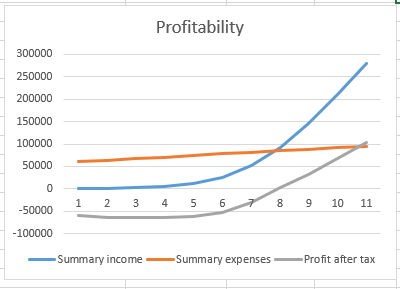
\includegraphics[width=0.5\textwidth]{figures/breakeven_no_salary.png}
    \caption{Breakeven point not including founder's personal cost}
    \label{fig:breakeven_no_salary}
\end{figure}

\begin{figure}[H]
    \centering
    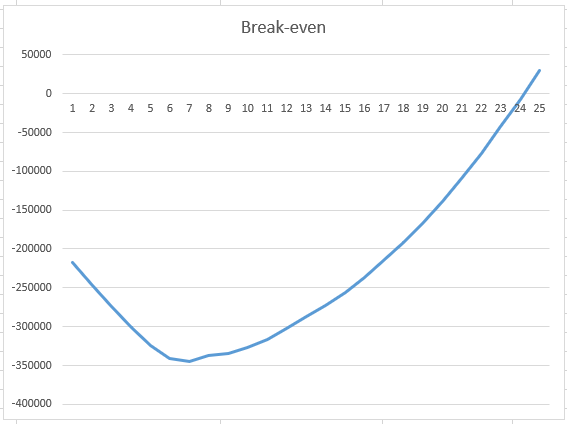
\includegraphics[width=0.5\textwidth]{figures/breakeven_salary.png}
    \caption{Breakeven point including founder's personal cost}
    \label{fig:breakeven_salary}
\end{figure}